% INTEL LAB DATA

We also evaluated our outlier detection framework on sensor data from the publicly available Intel Lab Data set \footnote{http://db.csail.mit.edu/labdata/labdata.html}. The Intel Lab Data contains data collected from 54 sensors spread throughout the Intel Berkeley Research Lab. Each data entry contains information including humidity, temperature, light and voltage taken from a Micro2dot sensor and weatherboard. The dataset contains a total of approximately 2.3 million measurements.

The Intel lab dataset has known outliers from faulty sensor readings due to periods of critically low voltage.
During these periods, the sensors go haywire and produce faulty measurements.

Due to the numerical nature of this data, the Simple Gaussian and Mixture models are well suited to analyzing it. However, the Histogram model does not fare as well.

% Random Sample 1000 data points
We analyze a sample of 1000 data points selected at random from the data set. Figure~\ref{fig:sensors_1k_gm} shows the results from the GM comparing voltage and temperature.
We parameterized the GM with a tolerance $\epsilon$ of 2.
Since the GM does not use correlation hints, the threshold for the statistical analyzer does not matter.

We observe that while the GM is able to detect the high and low voltage outliers, it also identifies points within the main cluster of the data between 20 and 30 Celsius.
These outliers are primarily due to light measurements whose measurements fall above 2 standard deviations above the norm.
When only outliers from temperature and voltage are taken into account, the outliers fall on the highest and lowest temperatures, as expected.

Figure~\ref{fig:sensors_1k_mm} shows the MM results for the same 1000 randomly-selected data points.
We use 0.75 as the threshold to determine correlation, 3 Gaussians to populate our model, and return 17\% of the data as outliers.

The statistical analyzer produces two correlations: between temperature and voltage with an $R$ coefficient of -0.75 and between temperature and humidity with an $R$ of -0.8.
The resulting MM produces outliers that register temperatures of over 120 degrees.
The points in the main cluster are the result of points that deviate from the correlation between temperature and humidity.

\begin{figure}[h]
\centering
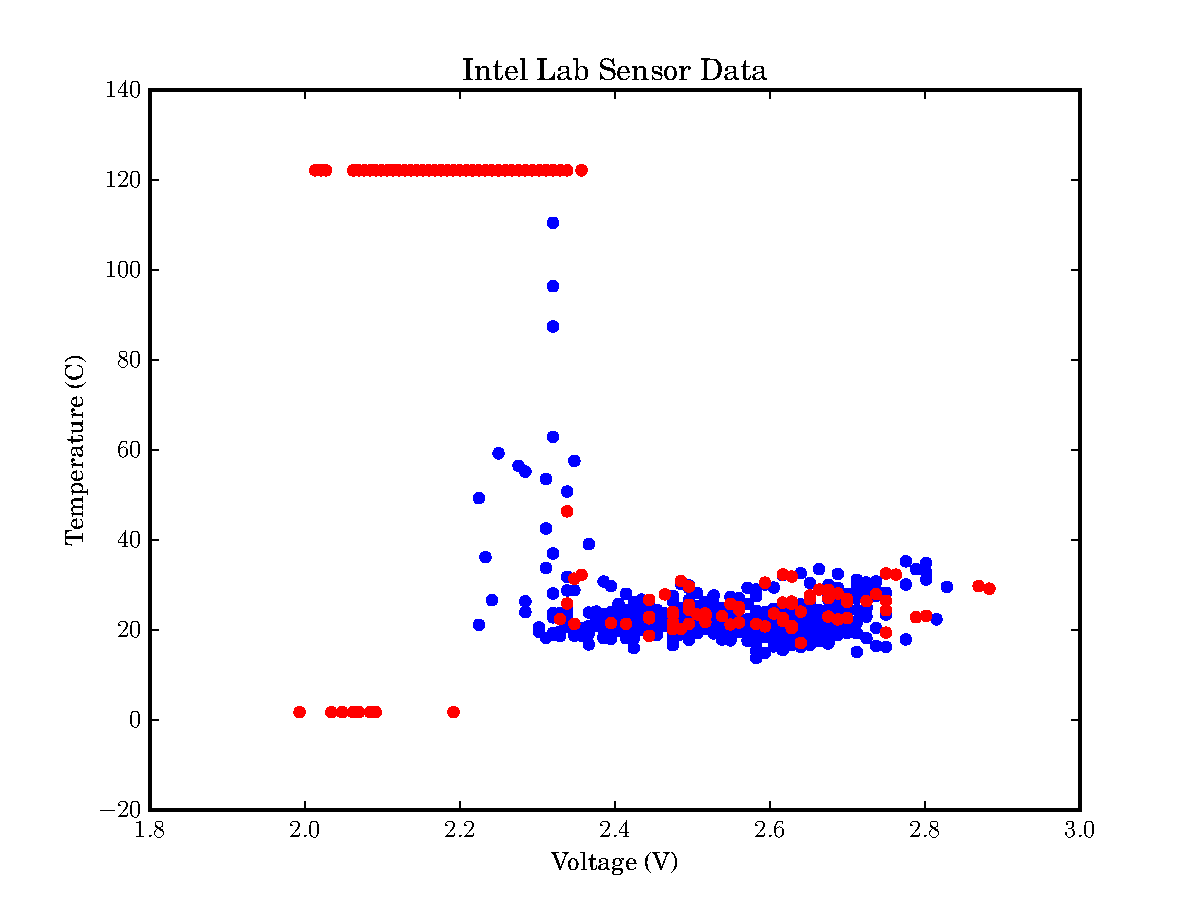
\includegraphics[width=0.45\textwidth]{../graphics/sensors_gm.pdf}
\caption{Outliers from sensor data detected by a Gaussian model.}
\label{fig:sensors_1k_gm}
\end{figure}
\begin{figure}[h]
\centering
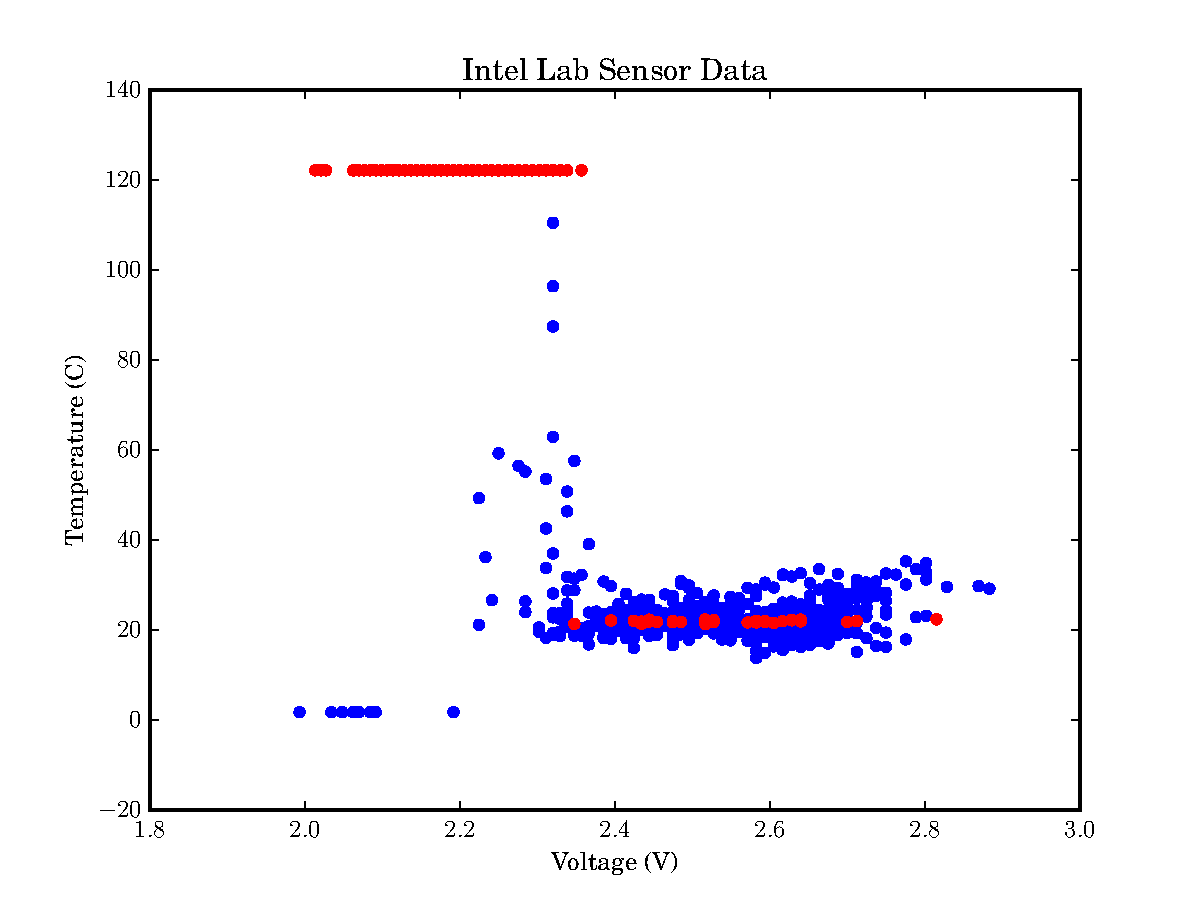
\includegraphics[width=0.45\textwidth]{../graphics/sensors_mm.pdf}
\caption{Outliers from sensor data detected by a Mixture model.}
\label{fig:sensors_1k_mm}
\end{figure}
